\documentclass[11pt,]{article}
\usepackage[]{mathpazo}
\usepackage{amssymb,amsmath}
\usepackage{ifxetex,ifluatex}
\usepackage{fixltx2e} % provides \textsubscript
\ifnum 0\ifxetex 1\fi\ifluatex 1\fi=0 % if pdftex
  \usepackage[T1]{fontenc}
  \usepackage[utf8]{inputenc}
\else % if luatex or xelatex
  \ifxetex
    \usepackage{mathspec}
  \else
    \usepackage{fontspec}
  \fi
  \defaultfontfeatures{Ligatures=TeX,Scale=MatchLowercase}
\fi
% use upquote if available, for straight quotes in verbatim environments
\IfFileExists{upquote.sty}{\usepackage{upquote}}{}
% use microtype if available
\IfFileExists{microtype.sty}{%
\usepackage{microtype}
\UseMicrotypeSet[protrusion]{basicmath} % disable protrusion for tt fonts
}{}
\usepackage[margin=1in]{geometry}
\usepackage{hyperref}
\hypersetup{unicode=true,
            pdftitle={Taxonomic assignment of endophytic isolate E14504F},
            pdfauthor={Dan Spakowicz},
            pdfborder={0 0 0},
            breaklinks=true}
\urlstyle{same}  % don't use monospace font for urls
\usepackage{natbib}
\bibliographystyle{plainnat}
\usepackage{color}
\usepackage{fancyvrb}
\newcommand{\VerbBar}{|}
\newcommand{\VERB}{\Verb[commandchars=\\\{\}]}
\DefineVerbatimEnvironment{Highlighting}{Verbatim}{commandchars=\\\{\}}
% Add ',fontsize=\small' for more characters per line
\usepackage{framed}
\definecolor{shadecolor}{RGB}{248,248,248}
\newenvironment{Shaded}{\begin{snugshade}}{\end{snugshade}}
\newcommand{\KeywordTok}[1]{\textcolor[rgb]{0.13,0.29,0.53}{\textbf{{#1}}}}
\newcommand{\DataTypeTok}[1]{\textcolor[rgb]{0.13,0.29,0.53}{{#1}}}
\newcommand{\DecValTok}[1]{\textcolor[rgb]{0.00,0.00,0.81}{{#1}}}
\newcommand{\BaseNTok}[1]{\textcolor[rgb]{0.00,0.00,0.81}{{#1}}}
\newcommand{\FloatTok}[1]{\textcolor[rgb]{0.00,0.00,0.81}{{#1}}}
\newcommand{\ConstantTok}[1]{\textcolor[rgb]{0.00,0.00,0.00}{{#1}}}
\newcommand{\CharTok}[1]{\textcolor[rgb]{0.31,0.60,0.02}{{#1}}}
\newcommand{\SpecialCharTok}[1]{\textcolor[rgb]{0.00,0.00,0.00}{{#1}}}
\newcommand{\StringTok}[1]{\textcolor[rgb]{0.31,0.60,0.02}{{#1}}}
\newcommand{\VerbatimStringTok}[1]{\textcolor[rgb]{0.31,0.60,0.02}{{#1}}}
\newcommand{\SpecialStringTok}[1]{\textcolor[rgb]{0.31,0.60,0.02}{{#1}}}
\newcommand{\ImportTok}[1]{{#1}}
\newcommand{\CommentTok}[1]{\textcolor[rgb]{0.56,0.35,0.01}{\textit{{#1}}}}
\newcommand{\DocumentationTok}[1]{\textcolor[rgb]{0.56,0.35,0.01}{\textbf{\textit{{#1}}}}}
\newcommand{\AnnotationTok}[1]{\textcolor[rgb]{0.56,0.35,0.01}{\textbf{\textit{{#1}}}}}
\newcommand{\CommentVarTok}[1]{\textcolor[rgb]{0.56,0.35,0.01}{\textbf{\textit{{#1}}}}}
\newcommand{\OtherTok}[1]{\textcolor[rgb]{0.56,0.35,0.01}{{#1}}}
\newcommand{\FunctionTok}[1]{\textcolor[rgb]{0.00,0.00,0.00}{{#1}}}
\newcommand{\VariableTok}[1]{\textcolor[rgb]{0.00,0.00,0.00}{{#1}}}
\newcommand{\ControlFlowTok}[1]{\textcolor[rgb]{0.13,0.29,0.53}{\textbf{{#1}}}}
\newcommand{\OperatorTok}[1]{\textcolor[rgb]{0.81,0.36,0.00}{\textbf{{#1}}}}
\newcommand{\BuiltInTok}[1]{{#1}}
\newcommand{\ExtensionTok}[1]{{#1}}
\newcommand{\PreprocessorTok}[1]{\textcolor[rgb]{0.56,0.35,0.01}{\textit{{#1}}}}
\newcommand{\AttributeTok}[1]{\textcolor[rgb]{0.77,0.63,0.00}{{#1}}}
\newcommand{\RegionMarkerTok}[1]{{#1}}
\newcommand{\InformationTok}[1]{\textcolor[rgb]{0.56,0.35,0.01}{\textbf{\textit{{#1}}}}}
\newcommand{\WarningTok}[1]{\textcolor[rgb]{0.56,0.35,0.01}{\textbf{\textit{{#1}}}}}
\newcommand{\AlertTok}[1]{\textcolor[rgb]{0.94,0.16,0.16}{{#1}}}
\newcommand{\ErrorTok}[1]{\textcolor[rgb]{0.64,0.00,0.00}{\textbf{{#1}}}}
\newcommand{\NormalTok}[1]{{#1}}
\usepackage{graphicx,grffile}
\makeatletter
\def\maxwidth{\ifdim\Gin@nat@width>\linewidth\linewidth\else\Gin@nat@width\fi}
\def\maxheight{\ifdim\Gin@nat@height>\textheight\textheight\else\Gin@nat@height\fi}
\makeatother
% Scale images if necessary, so that they will not overflow the page
% margins by default, and it is still possible to overwrite the defaults
% using explicit options in \includegraphics[width, height, ...]{}
\setkeys{Gin}{width=\maxwidth,height=\maxheight,keepaspectratio}
\IfFileExists{parskip.sty}{%
\usepackage{parskip}
}{% else
\setlength{\parindent}{0pt}
\setlength{\parskip}{6pt plus 2pt minus 1pt}
}
\setlength{\emergencystretch}{3em}  % prevent overfull lines
\providecommand{\tightlist}{%
  \setlength{\itemsep}{0pt}\setlength{\parskip}{0pt}}
\setcounter{secnumdepth}{0}
% Redefines (sub)paragraphs to behave more like sections
\ifx\paragraph\undefined\else
\let\oldparagraph\paragraph
\renewcommand{\paragraph}[1]{\oldparagraph{#1}\mbox{}}
\fi
\ifx\subparagraph\undefined\else
\let\oldsubparagraph\subparagraph
\renewcommand{\subparagraph}[1]{\oldsubparagraph{#1}\mbox{}}
\fi

%%% Use protect on footnotes to avoid problems with footnotes in titles
\let\rmarkdownfootnote\footnote%
\def\footnote{\protect\rmarkdownfootnote}

%%% Change title format to be more compact
\usepackage{titling}

% Create subtitle command for use in maketitle
\newcommand{\subtitle}[1]{
  \posttitle{
    \begin{center}\large#1\end{center}
    }
}

\setlength{\droptitle}{-2em}
  \title{Taxonomic assignment of endophytic isolate E14504F}
  \pretitle{\vspace{\droptitle}\centering\huge}
  \posttitle{\par}
  \author{Dan Spakowicz}
  \preauthor{\centering\large\emph}
  \postauthor{\par}
  \predate{\centering\large\emph}
  \postdate{\par}
  \date{May 11, 2017}


\begin{document}
\maketitle

\section{Introduction}\label{introduction}

This is the script used to build a tree for Nneoma's fungus and assign
its taxonomy.

I started by rolling through the databases from the recent review
\url{http://jcm.asm.org/content/55/4/1011.full} to check if any would be
useful for this project.

\begin{itemize}
\tightlist
\item
  BOLD systems
  \url{http://v4.boldsystems.org/index.php/IDS_OpenIdEngine} only have
  ITS identification.
\item
  Looks like this is a good place for morphological features
  \url{https://aftol.umn.edu/} and can even make a nexus file to include
  in the tree -- but aftol has been lost? (goes to godaddy
  website\ldots{})
\item
  BROAD doesn't have an identification portal
\item
  EZBioCloud doesn't have a fungal id section
\item
  FungiDB is just genomics
\item
  UNITE is just ITS
\item
  IndexFungorum doesn't have an id search (but could be useful for
  morphology)
\item
  CBS can be searched directly for LSU and there are lots of good hits.
  However, I'd rather find a paper that has gone through the effort of
  identifying isolates with multiple loci
\item
  SILVA has an LSU search \url{https://www.arb-silva.de/}
\item
  Identity: 43.61, LCA tax SILVA: None
\item
  SSU Iden: 99.37, LCA tax. SILVA: None
\item
  RDP \url{http://rdp.cme.msu.edu/classifier/}
\item
  E14504F-LSU Root(100\%) Fungi(100\%) Basidiomycota(100\%)
  Agaricomycetes(100\%) Cantharellales(100\%) Ceratobasidiaceae(100\%)
  Thanatephorus(100\%)
\end{itemize}

The RDP result is strong, with 100\% confidence in the genus
Thanatephorus. The CBS searches also found organisms of either
Thanatephorus (telomorph) or Rhizoctonia (anamorph). This will very
likely be the genus to which E14504F belongs. In addition, Nneoma and I
found a few papers that deal with isolates of Rhizoctonia/Thanatephorus:

\begin{itemize}
\tightlist
\item
  \citep{gonzalez_ribosomal_2001} has a bunch of Thanatephorus isolates
  with genbank accession numbers for ITS and 28S, but nothing outside
  the genus (which is necessary to demonstrate the circumscription in
  this case).
\item
  \citep{tupac_otero_diversity_2002} just have ITS and have several
  genera that were isolated from orchids. It's more orchid-centric than
  fungus-centric.
\item
  \citep{lopez-chavez_proteomic_2016} defines a Thanatephorus isolate
  using ITS alone. The tree shows weak node support separating
  Thanatephorus from Ceratobasidium, but clearly their isolate is
  closest to a Thana.
\item
  \citep{gonzalez_phylogenetic_2016} does a really nice job of creating
  a multi-locus tree. This should be the model going forward.
\end{itemize}

\section{Methods}\label{methods}

I converted the table of genbank accession numbers from
\citep{gonzalez_phylogenetic_2016} to a google spreadsheet.

Here are the files that Nneoma created using the Staden package (pregap
\& gap). As soon as these have genbank accession numbers I'll add them
to the table so that they can be pulled with the other sequences from
the table and remove this code block and the merge code block.

\begin{Shaded}
\begin{Highlighting}[]
\NormalTok{files <-}\StringTok{ }\KeywordTok{list.files}\NormalTok{(}\DataTypeTok{path =} \StringTok{"~/Dropbox/Rainforest project/E14504F sequences/"}\NormalTok{, }\DataTypeTok{pattern =} \StringTok{"*.fasta"}\NormalTok{, }\DataTypeTok{full.names =} \OtherTok{TRUE}\NormalTok{)}
\NormalTok{ofastas <-}\StringTok{ }\KeywordTok{list}\NormalTok{()}
\NormalTok{for (f in files) \{}
  \NormalTok{tmp <-}\StringTok{ }\KeywordTok{readLines}\NormalTok{(f)}
  \NormalTok{tmp[}\DecValTok{2}\NormalTok{:}\KeywordTok{length}\NormalTok{(tmp)] <-}\StringTok{ }\KeywordTok{toupper}\NormalTok{(tmp[}\DecValTok{2}\NormalTok{:}\KeywordTok{length}\NormalTok{(tmp)])}
  \NormalTok{ofastas[[f]] <-}\StringTok{ }\NormalTok{tmp}
\NormalTok{\}}

\CommentTok{# Adjust names of list}
\NormalTok{CleanPaths <-}\StringTok{ }\NormalTok{function(names)\{}
  \NormalTok{tmp <-}\StringTok{ }\KeywordTok{gsub}\NormalTok{(}\StringTok{".*E14504F? (.*)}\CharTok{\textbackslash{}\textbackslash{}}\StringTok{.fasta"}\NormalTok{, }\StringTok{"}\CharTok{\textbackslash{}\textbackslash{}}\StringTok{1"}\NormalTok{, names)}
  \NormalTok{tmp <-}\StringTok{ }\KeywordTok{gsub}\NormalTok{(}\StringTok{" partial| FULL| ver2"}\NormalTok{, }\StringTok{"}\CharTok{\textbackslash{}\textbackslash{}}\StringTok{1"}\NormalTok{, tmp)}
  \KeywordTok{return}\NormalTok{(tmp)}
\NormalTok{\}}
\NormalTok{names <-}\StringTok{ }\KeywordTok{CleanPaths}\NormalTok{(}\KeywordTok{names}\NormalTok{(ofastas))}
\KeywordTok{names}\NormalTok{(ofastas) <-}\StringTok{ }\NormalTok{names}

\CommentTok{# Cat ITS1 and ITS2 sep by 100 N's and remove ITS2}
\NormalTok{its <-}\StringTok{ }\KeywordTok{grep}\NormalTok{(}\StringTok{"ITS"}\NormalTok{, }\KeywordTok{names}\NormalTok{(ofastas))}
\NormalTok{ofastas[[its[}\DecValTok{1}\NormalTok{]]] <-}\StringTok{ }\KeywordTok{c}\NormalTok{(ofastas[[its[}\DecValTok{1}\NormalTok{]]], }\KeywordTok{paste}\NormalTok{(}\KeywordTok{rep}\NormalTok{(}\StringTok{"N"}\NormalTok{, }\DecValTok{100}\NormalTok{), }\DataTypeTok{collapse =} \StringTok{""}\NormalTok{), ofastas[[its[}\DecValTok{2}\NormalTok{]]][}\DecValTok{2}\NormalTok{])}
\NormalTok{ofastas <-}\StringTok{ }\NormalTok{ofastas[-its[}\DecValTok{2}\NormalTok{]]}
\KeywordTok{names}\NormalTok{(ofastas)[}\KeywordTok{grep}\NormalTok{(}\StringTok{"ITS"}\NormalTok{, }\KeywordTok{names}\NormalTok{(ofastas))] <-}\StringTok{ "ITS"}
\end{Highlighting}
\end{Shaded}

\begin{Shaded}
\begin{Highlighting}[]
\CommentTok{# Load table into dataframe}
\NormalTok{sheet <-}\StringTok{ }\KeywordTok{gs_title}\NormalTok{(}\StringTok{"E14504F"}\NormalTok{)}
\NormalTok{x <-}\StringTok{ }\KeywordTok{gs_read}\NormalTok{(sheet)}

\CommentTok{# Convert hyphen-only columns to NA}
\NormalTok{x <-}\StringTok{ }\KeywordTok{data.frame}\NormalTok{(}\KeywordTok{apply}\NormalTok{(x, }\DecValTok{2}\NormalTok{, function(x) }\KeywordTok{gsub}\NormalTok{(}\StringTok{"^-$"}\NormalTok{, }\OtherTok{NA}\NormalTok{, x)), }\DataTypeTok{as.is =} \OtherTok{TRUE}\NormalTok{)}

\CommentTok{# Take in a character vector of genbank accession numbers and return a fasta file in ape format}
\NormalTok{RetrieveSequencesAsString <-}\StringTok{ }\NormalTok{function(charvec)\{}
  \KeywordTok{try}\NormalTok{(\{}
    \NormalTok{string <-}\StringTok{ }\KeywordTok{entrez_fetch}\NormalTok{(}\DataTypeTok{db =} \StringTok{"nucleotide"}\NormalTok{, }\DataTypeTok{id =} \NormalTok{charvec, }\DataTypeTok{rettype =} \StringTok{"fasta"}\NormalTok{)}
    \NormalTok{string <-}\StringTok{ }\KeywordTok{unlist}\NormalTok{(}\KeywordTok{strsplit}\NormalTok{(string, }\DataTypeTok{split =} \StringTok{"}\CharTok{\textbackslash{}n}\StringTok{"}\NormalTok{))}
    \KeywordTok{return}\NormalTok{(string)}
  \NormalTok{\}, }\DataTypeTok{silent =} \OtherTok{TRUE}\NormalTok{)}
\NormalTok{\}}

\CommentTok{# Retrieve all sequence into a list}
\NormalTok{loci <-}\StringTok{ }\KeywordTok{colnames}\NormalTok{(x[,}\DecValTok{5}\NormalTok{:}\DecValTok{11}\NormalTok{])}
\NormalTok{gfastas <-}\StringTok{ }\KeywordTok{list}\NormalTok{()}
\NormalTok{for (i in loci) \{}
  \NormalTok{gfastas[[i]] <-}\StringTok{ }\KeywordTok{RetrieveSequencesAsString}\NormalTok{(x[,}\KeywordTok{grep}\NormalTok{(i, }\KeywordTok{colnames}\NormalTok{(x))])}
\NormalTok{\}}
\CommentTok{# Remove those without any sequences}
\NormalTok{gfastas <-}\StringTok{ }\NormalTok{gfastas[-(}\KeywordTok{which}\NormalTok{(}\KeywordTok{sapply}\NormalTok{(gfastas, class) ==}\StringTok{ "try-error"}\NormalTok{))]}
\end{Highlighting}
\end{Shaded}

\begin{Shaded}
\begin{Highlighting}[]
\NormalTok{bfastas <-}\StringTok{ }\KeywordTok{list}\NormalTok{()}
\NormalTok{for (n in }\KeywordTok{names}\NormalTok{(gfastas))\{}
  \NormalTok{if (n %in%}\StringTok{ }\KeywordTok{names}\NormalTok{(ofastas)) \{}
    \NormalTok{bfastas[[n]] <-}\StringTok{ }\KeywordTok{c}\NormalTok{(gfastas[[n]], ofastas[[}\KeywordTok{which}\NormalTok{(}\KeywordTok{names}\NormalTok{(ofastas) %in%}\StringTok{ }\NormalTok{n)]])}
  \NormalTok{\} else \{}
    \NormalTok{bfastas[[n]] <-}\StringTok{ }\NormalTok{gfastas[[n]]}
  \NormalTok{\}}
\NormalTok{\}}
\end{Highlighting}
\end{Shaded}

\begin{Shaded}
\begin{Highlighting}[]
\CommentTok{# Read in each string as a fasta file}
\NormalTok{fastas <-}\StringTok{ }\KeywordTok{list}\NormalTok{()}
\NormalTok{for (i in }\DecValTok{1}\NormalTok{:}\KeywordTok{length}\NormalTok{(bfastas)) \{}
  \NormalTok{temp <-}\StringTok{ }\KeywordTok{tempfile}\NormalTok{()}
  \KeywordTok{write}\NormalTok{(bfastas[[i]], temp)}
  \NormalTok{fastas[[i]] <-}\StringTok{ }\KeywordTok{read.FASTA}\NormalTok{(}\DataTypeTok{file =} \NormalTok{temp)}
\NormalTok{\}}

\CommentTok{# Align sequences}
\NormalTok{alns <-}\StringTok{ }\KeywordTok{lapply}\NormalTok{(fastas, ape::muscle)}

\CommentTok{# Remove gaps present in 30% of the columns}
\NormalTok{rmgaps <-}\StringTok{ }\KeywordTok{lapply}\NormalTok{(alns, function(x) }\KeywordTok{del.colgapsonly}\NormalTok{(x, }\DataTypeTok{threshold =} \FloatTok{0.3}\NormalTok{))}
\KeywordTok{names}\NormalTok{(rmgaps) <-}\StringTok{ }\KeywordTok{names}\NormalTok{(bfastas)}
\end{Highlighting}
\end{Shaded}

\begin{Shaded}
\begin{Highlighting}[]
\KeywordTok{lapply}\NormalTok{(rmgaps, function(x) }\KeywordTok{image.DNAbin}\NormalTok{(x, }\DataTypeTok{show.labels =} \OtherTok{FALSE}\NormalTok{))}
\end{Highlighting}
\end{Shaded}

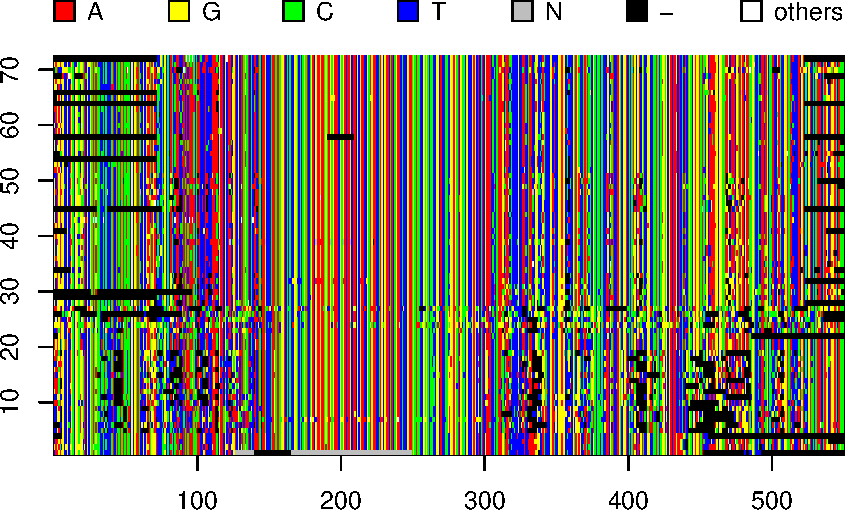
\includegraphics{DS_tree_files/figure-latex/visualize alignments-1.pdf}
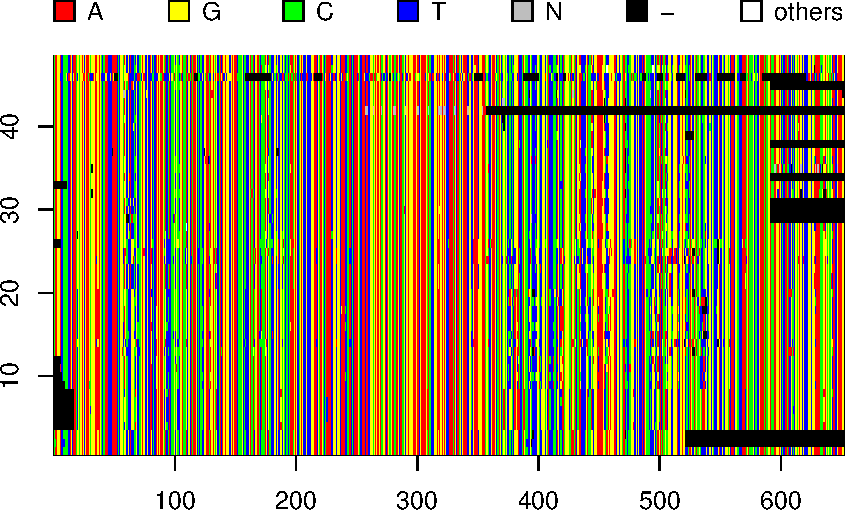
\includegraphics{DS_tree_files/figure-latex/visualize alignments-2.pdf}
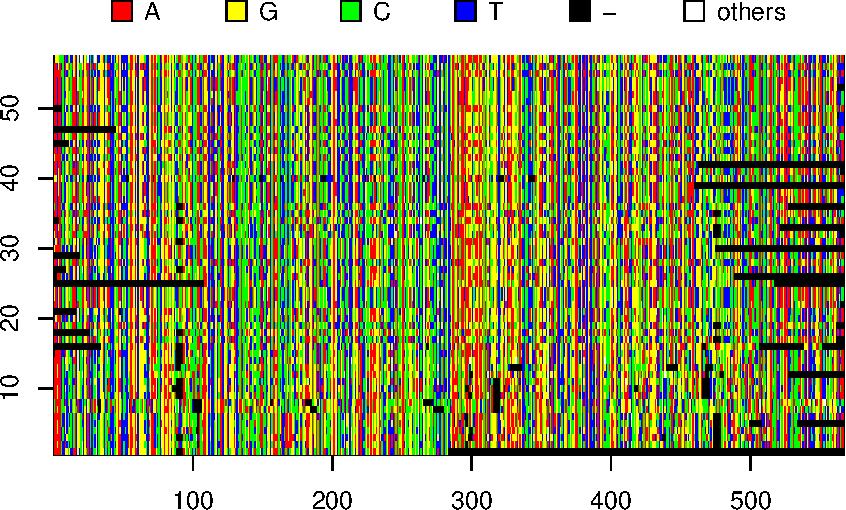
\includegraphics{DS_tree_files/figure-latex/visualize alignments-3.pdf}
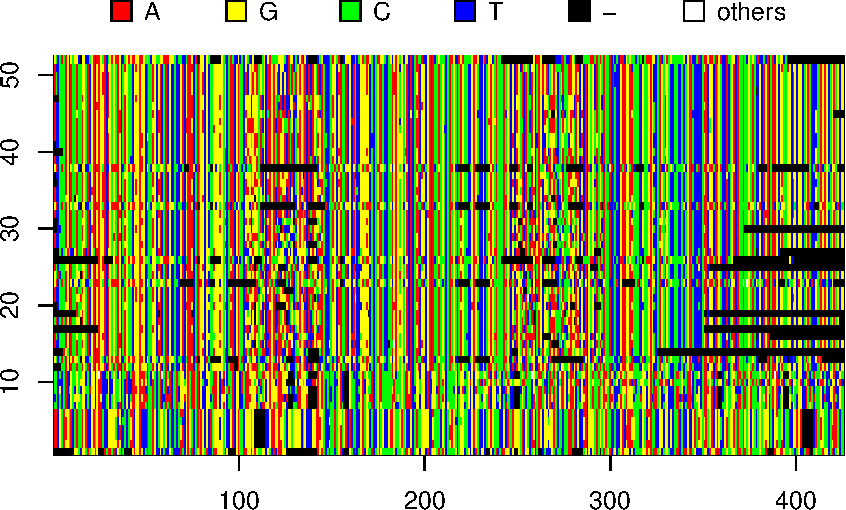
\includegraphics{DS_tree_files/figure-latex/visualize alignments-4.pdf}
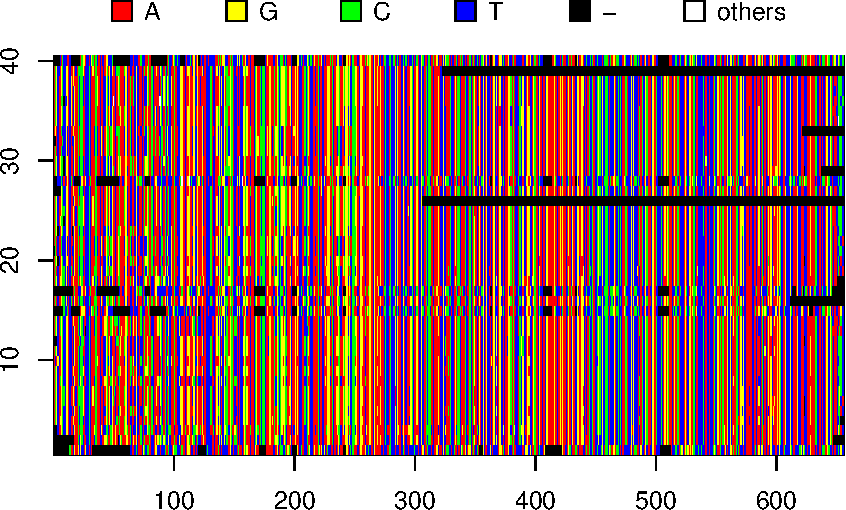
\includegraphics{DS_tree_files/figure-latex/visualize alignments-5.pdf}

\begin{verbatim}
## $ITS
## $ITS$rect
## $ITS$rect$w
## [1] 565.4039
## 
## $ITS$rect$h
## [1] 10.82707
## 
## $ITS$rect$left
## [1] -7.951949
## 
## $ITS$rect$top
## [1] 85.99098
## 
## 
## $ITS$text
## $ITS$text$x
## [1]  23.35984 103.01355 182.66725 262.32096 341.97467 421.62837 501.28208
## 
## $ITS$text$y
## [1] 80.57745 80.57745 80.57745 80.57745 80.57745 80.57745 80.57745
## 
## 
## 
## $LSU
## $LSU$rect
## $LSU$rect$w
## [1] 670.4516
## 
## $LSU$rect$h
## [1] 7.218045
## 
## $LSU$rect$left
## [1] -9.475808
## 
## $LSU$rect$top
## [1] 57.51256
## 
## 
## $LSU$text
## $LSU$text$x
## [1]  27.65347 122.10623 216.55898 311.01174 405.46450 499.91725 594.37001
## 
## $LSU$text$y
## [1] 53.90353 53.90353 53.90353 53.90353 53.90353 53.90353 53.90353
## 
## 
## 
## $RPB2
## $RPB2$rect
## $RPB2$rect$w
## [1] 500.7916
## 
## $RPB2$rect$h
## [1] 8.571429
## 
## $RPB2$rect$left
## [1] 32.85418
## 
## $RPB2$rect$top
## [1] 68.19196
## 
## 
## $RPB2$text
## $RPB2$text$x
## [1]  65.13555 147.25577 229.37598 311.49620 393.61641 475.73663
## 
## $RPB2$text$y
## [1] 63.90625 63.90625 63.90625 63.90625 63.90625 63.90625
## 
## 
## 
## $TEF1
## $TEF1$rect
## $TEF1$rect$w
## [1] 376.0361
## 
## $TEF1$rect$h
## [1] 7.819549
## 
## $TEF1$rect$left
## [1] 24.73194
## 
## $TEF1$rect$top
## [1] 62.25896
## 
## 
## $TEF1$text
## $TEF1$text$x
## [1]  48.97148 110.63419 172.29689 233.95960 295.62231 357.28501
## 
## $TEF1$text$y
## [1] 58.34918 58.34918 58.34918 58.34918 58.34918 58.34918
## 
## 
## 
## $ATP6
## $ATP6$rect
## $ATP6$rect$w
## [1] 579.538
## 
## $ATP6$rect$h
## [1] 6.015038
## 
## $ATP6$rect$left
## [1] 37.98099
## 
## $ATP6$rect$top
## [1] 48.01975
## 
## 
## $ATP6$text
## $ATP6$text$x
## [1]  75.3384 170.3715 265.4046 360.4377 455.4708 550.5040
## 
## $ATP6$text$y
## [1] 45.01223 45.01223 45.01223 45.01223 45.01223 45.01223
\end{verbatim}

I can't figure out how to add titles in \texttt{image.DNAbin()}, but the
order is ``ITS'' ``LSU'' ``RPB2'' ``TEF1'' ``ATP6''. The ITS looks to
have a few orgs that might be revcomps, maybe three. I'm not sure how
best to identify those and replace them in this format. It looks like
the N length is short by \textasciitilde{} 20nt.

\subsection{Alternative methods}\label{alternative-methods}

\begin{itemize}
\tightlist
\item
  retreive Treebase file and add E14504F sequences to those alignments
\item
  This is becomeing increasingly attractive given the seemingly large
  fraction of reverse complements observed. Particularly now that the
  ITS1 and ITS2 sequences are available, all sections except atp6 would
  be usable. It's worth taking the time to explore how to add one more
  sequence onto an existing alignment in R.
\end{itemize}

\begin{Shaded}
\begin{Highlighting}[]
\KeywordTok{search_treebase}\NormalTok{()}
\end{Highlighting}
\end{Shaded}

\section{Results and Discussion}\label{results-and-discussion}

\renewcommand\refname{References}
\bibliography{Nneoma.bib}


\end{document}
